\documentclass[border=12pt]{standalone}
\usepackage{amsmath}
\usepackage{tikz}
\usetikzlibrary{positioning, arrows.meta, calc, fit, backgrounds, shapes.geometric}
\begin{document}
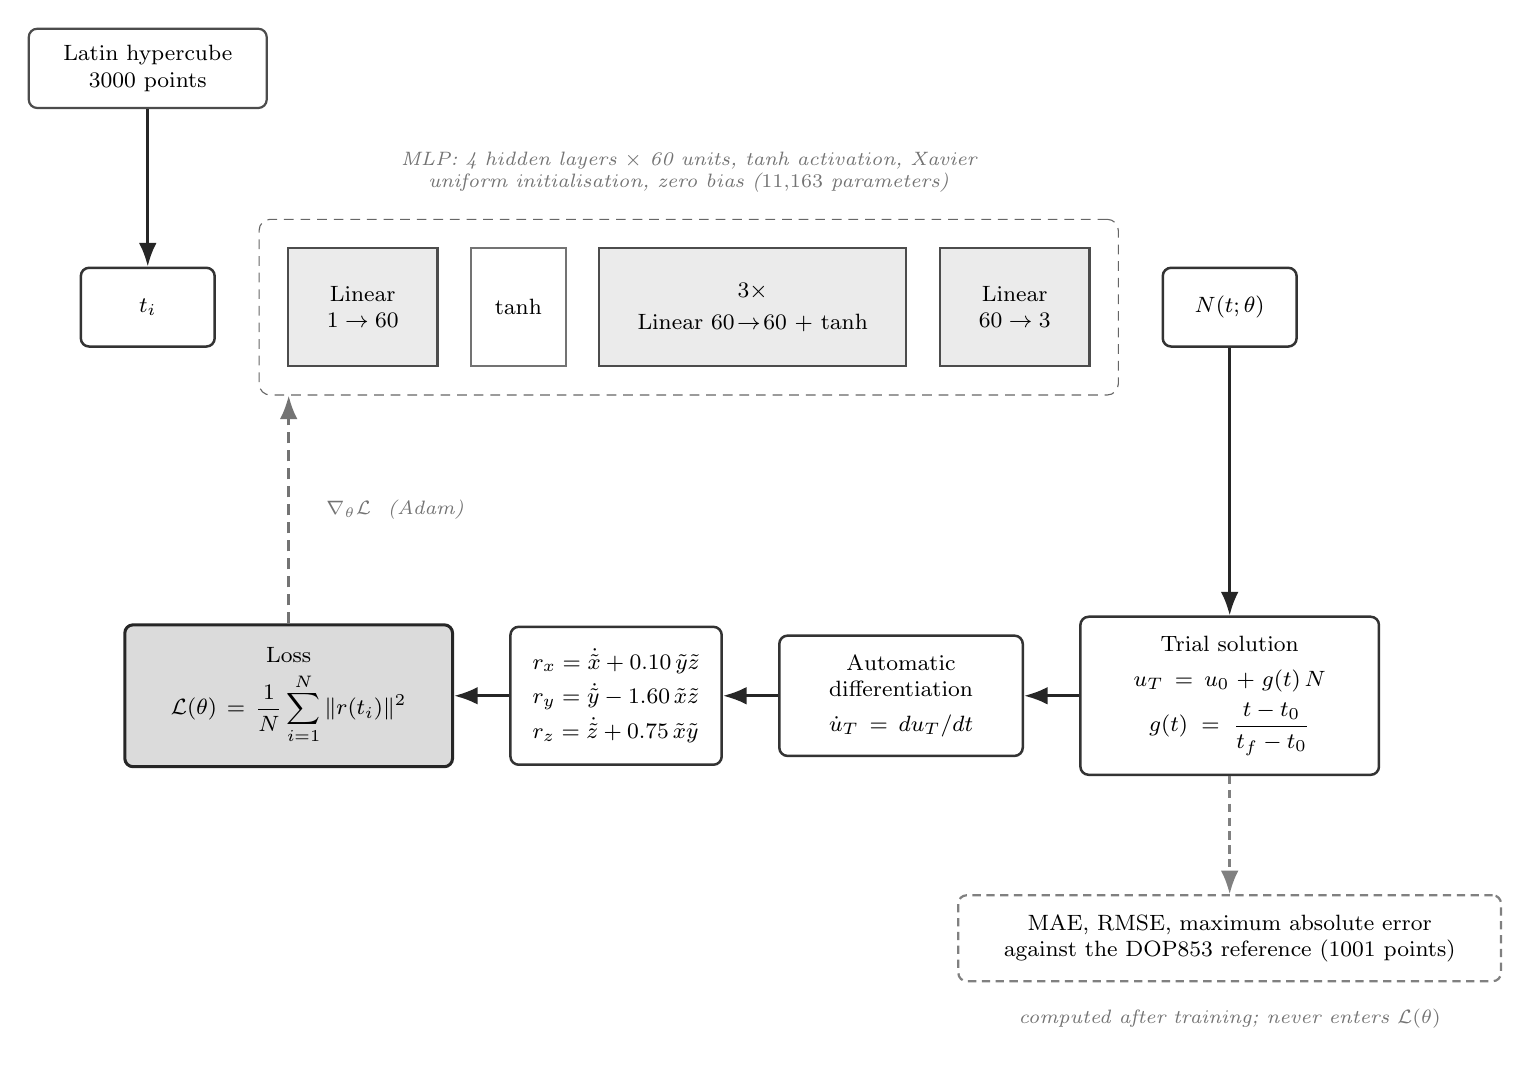
\begin{tikzpicture}[
    font=\footnotesize,
    io/.style={rounded corners=3pt, draw=black!80, fill=white, line width=0.9pt,
               align=center, inner sep=6pt, minimum height=1.0cm, minimum width=1.7cm},
    lay/.style={draw=black!70, fill=black!8, line width=0.8pt, align=center,
                inner sep=5pt, minimum height=1.5cm, minimum width=1.9cm},
    act/.style={draw=black!55, fill=white, line width=0.7pt, align=center,
                inner sep=5pt, minimum height=1.5cm, minimum width=1.2cm},
    rep/.style={draw=black!70, fill=black!8, line width=0.8pt, align=center,
                inner sep=5pt, minimum height=1.5cm, minimum width=3.9cm},
    proc/.style={rounded corners=3pt, draw=black!80, fill=white, line width=0.9pt,
                 align=center, inner sep=7pt, minimum height=1.5cm},
    res/.style={rounded corners=3pt, draw=black!80, fill=white, line width=0.9pt,
                align=left, inner sep=8pt, minimum height=1.5cm},
    loss/.style={rounded corners=3pt, draw=black!85, fill=black!14, line width=1.1pt,
                 align=center, inner sep=8pt, minimum height=1.5cm},
    ev/.style={rounded corners=3pt, draw=black!50, fill=white, line width=0.8pt,
               align=center, inner sep=7pt, dash pattern=on 3pt off 2pt},
    samp/.style={rounded corners=3pt, draw=black!70, fill=white, line width=0.8pt,
                 align=center, inner sep=6pt, minimum height=1.0cm},
    flow/.style={-{Latex[length=3mm]}, line width=1.0pt, draw=black!85},
    back/.style={-{Latex[length=3mm]}, line width=1.0pt, draw=black!55,
                 dash pattern=on 4pt off 2.5pt},
    evflow/.style={-{Latex[length=3mm]}, line width=0.9pt, draw=black!50,
                   dash pattern=on 3pt off 2pt},
    note/.style={font=\scriptsize\itshape, text=black!55, align=center}
]

% ---------- input row ----------
\node[io] (t) {$t_i$};
\node[lay, right=0.9cm of t]   (l1)  {Linear\\$1 \to 60$};
\node[act, right=0.4cm of l1]  (a1)  {$\tanh$};
\node[rep, right=0.4cm of a1]  (mid) {$3\times$\\[2pt]Linear $60\!\to\!60$ $+$ $\tanh$};
\node[lay, right=0.4cm of mid] (lo)  {Linear\\$60 \to 3$};
\node[io,  right=0.9cm of lo]  (N)   {$N(t;\theta)$};

\begin{scope}[on background layer]
  \node[draw=black!60, dash pattern=on 3.5pt off 2.5pt, rounded corners=4pt,
        fit=(l1)(a1)(mid)(lo), inner sep=10pt] (netbox) {};
\end{scope}
\node[note, above=6pt of netbox, text width=12cm]
     {MLP: 4 hidden layers $\times$ 60 units, tanh activation,
      Xavier uniform initialisation, zero bias ($11{,}163$ parameters)};

% ---------- collocation sampler, above the input ----------
\node[samp, above=2.0cm of t, text width=2.6cm] (samp)
     {Latin hypercube\\$3000$ points};
\draw[flow] (samp) -- (t);

% ---------- lower band: placed left to right, traversed right to left ----------
\node[proc, below=3.4cm of N, text width=3.3cm] (trial)
     {Trial solution\\[3pt]$u_T = u_0 + g(t)\,N$\\[3pt]
      $g(t) = \dfrac{t - t_0}{t_f - t_0}$};
\node[proc, left=0.7cm of trial, text width=2.6cm] (ad)
     {Automatic\\differentiation\\[3pt]$\dot{u}_T = du_T/dt$};
\node[res, left=0.7cm of ad] (r)
     {$r_x = \dot{\tilde{x}} + 0.10\,\tilde{y}\tilde{z}$\\[3pt]
      $r_y = \dot{\tilde{y}} - 1.60\,\tilde{x}\tilde{z}$\\[3pt]
      $r_z = \dot{\tilde{z}} + 0.75\,\tilde{x}\tilde{y}$};
\node[loss, left=0.7cm of r, text width=3.6cm] (L)
     {Loss\\[3pt]$\mathcal{L}(\theta) = \dfrac{1}{N}\displaystyle\sum_{i=1}^{N}\|r(t_i)\|^2$};

\draw[flow] (N.south) -- (trial.north);
\draw[flow] (trial) -- (ad);
\draw[flow] (ad) -- (r);
\draw[flow] (r) -- (L);

% ---------- backward pass: vertical, label well clear of the line ----------
\draw[back] (L.north) -- (L.north |- netbox.south);
\node[note, right=10pt] at ($(L.north)!0.5!(L.north |- netbox.south)$)
     {$\nabla_\theta \mathcal{L}$ \ (Adam)};

% ---------- evaluation branch, deliberately detached ----------
\node[ev, below=1.5cm of trial, text width=6.4cm] (eval)
     {MAE, RMSE, maximum absolute error\\
      against the DOP853 reference ($1001$ points)};
\draw[evflow] (trial.south) -- (eval.north);
\node[note, below=6pt of eval, text width=6.0cm]
     {computed after training; never enters $\mathcal{L}(\theta)$};

\end{tikzpicture}
\end{document}
